% Copyright (c) 2014,2016,2018 Casper Ti. Vector
% Public domain.

\chapter{基于分层四叉树的地形高程编辑}
对地形高程数据的常见编辑操作包括对地形高程进行抬高和降低、平整地形、平滑地形、腐蚀地形和对地形数据中的坏点进行修复等。笔刷是进行高程编辑最基本的工具,使用笔刷对地形高程进行抬高和降低,构造山峰、丘陵、山谷等地形,是地形高程编辑的常用手段。除此之外,城市和机场等场景常通过平整操作来提供可信的地形环境,自然场景常通过模拟外部因素对地形的腐蚀作用,来增强地形的真实感。\par
\section{基于笔刷的地形高程编辑}
高程编辑的笔刷为圆形,笔刷的大小存在不动性,即随视角高度的变化笔刷覆盖的屏幕像素数不变。编辑时,鼠标采样点以经纬度形式表示,因此将笔刷直径大小也换算为经纬度参与编辑范围的运算。一系列笔刷绘制点两两之间生成一个多边形,框定在地形数据中参与编辑的像素,若干个多边形连起来形成笔迹。设笔刷直径为$t$,首先将相邻的两个鼠标采样点$A$和$B$投影到地平面上,分别找到通过$A$点和$B$点的绘制曲线的垂线,在这条垂线上向正方向和负方向分别取得与$A$点和$B$点距离$t/2$的点作为多边形的四个顶点。如图4.1所示,图中红色点分别为两个相邻的绘制点$A$和$B$,绿色点为多边形顶点,根据绿色点$x$、$y$坐标的最大和最小值,在图中用蓝色点标出。蓝色的外框划定了计算时所需要遍历的像素的范围,这些像素与多边形进行求交,得到最终被编辑操作修改的像素,并由浅绿色标出。\par

\begin{figure}[ht]
    \centering
    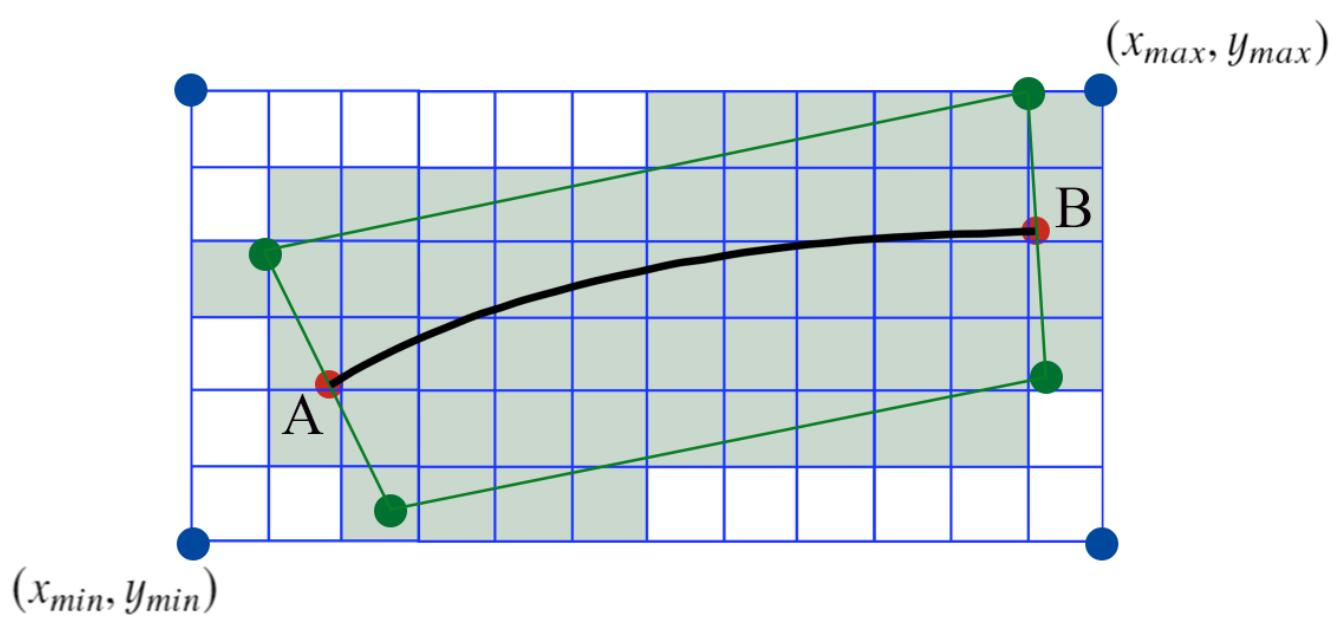
\includegraphics[height=4.7cm ,width=10.45cm]{figures/editArea.jpg}
  \caption{高程笔刷编辑范围}
  \end{figure}
设用户设定的笔刷的编辑高度为$H$,从笔刷中心向边缘,编辑高度逐渐降低,至笔刷边缘时降为0。对地形上某点$p$,其编辑高度$h(p)$由该点到距该点最近的绘制点的距离$d$和函数$f$决定:
\begin{equation}
h(p) = f \circ d(p)
\end{equation}
这里函数$f$选用了Wyvill field function\supercite{wyvill},其定义域和值域都为[0,1],并随着输入值增大,从1平滑的向0过渡。该计算将笔刷覆盖范围内每个点与绘制点的距离映射为编辑后高度与原始高度混合的权重,可以实现从笔刷中心点向笔刷边缘编辑高度平滑减小的效果,该函数如图4.2所示。\par
\begin{figure}[ht]
\centering
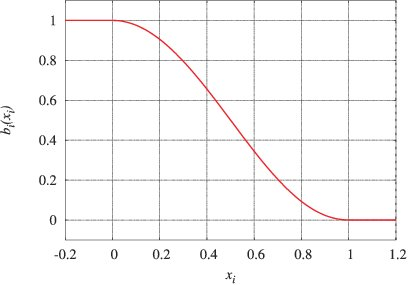
\includegraphics[height=4cm        ,width=5cm]{figures/Wyvill-field-function.jpg}
\caption{Wyvill Field Function\supercite{wyvill}}
\end{figure}
对补丁数据中的某点进行修改时的计算如下:首先从其中获取原始地形高度$h_{start}$,并获取笔迹曲线上离该点距离最近的一个绘制点,取其高度$h_{line}$。由该计算的定义方式可知,编辑结束后绘制点的高度变为其原始高度与$H$的和,记为$h_{end}$。依据$h_{start}$、$h_{end}$和$d(p)$,编辑后高度$h_{result}$为:\par
\begin{equation}
\begin{aligned}
& f(d(p)) = 3 * d(p)^2 - 2 * d(p)^3\\
&h_{result}=h_{start} * (1 - f(d(p))) + h_{end} * f(d(p))
\end{aligned}
\end{equation}
使用地形平整模式进行笔刷编辑时,可以额外设定笔刷硬度参数,该参数决定笔刷内直径与笔刷外直径的比例。笔刷内直径覆盖的面积内$f$的参数为0,即不参与与原始地形高度的混合,直接更新为用户所设置的高度值。笔刷内直径到笔刷外直径中间的部分按照$f$进行混合。\par
\begin{figure}[ht]
\centering
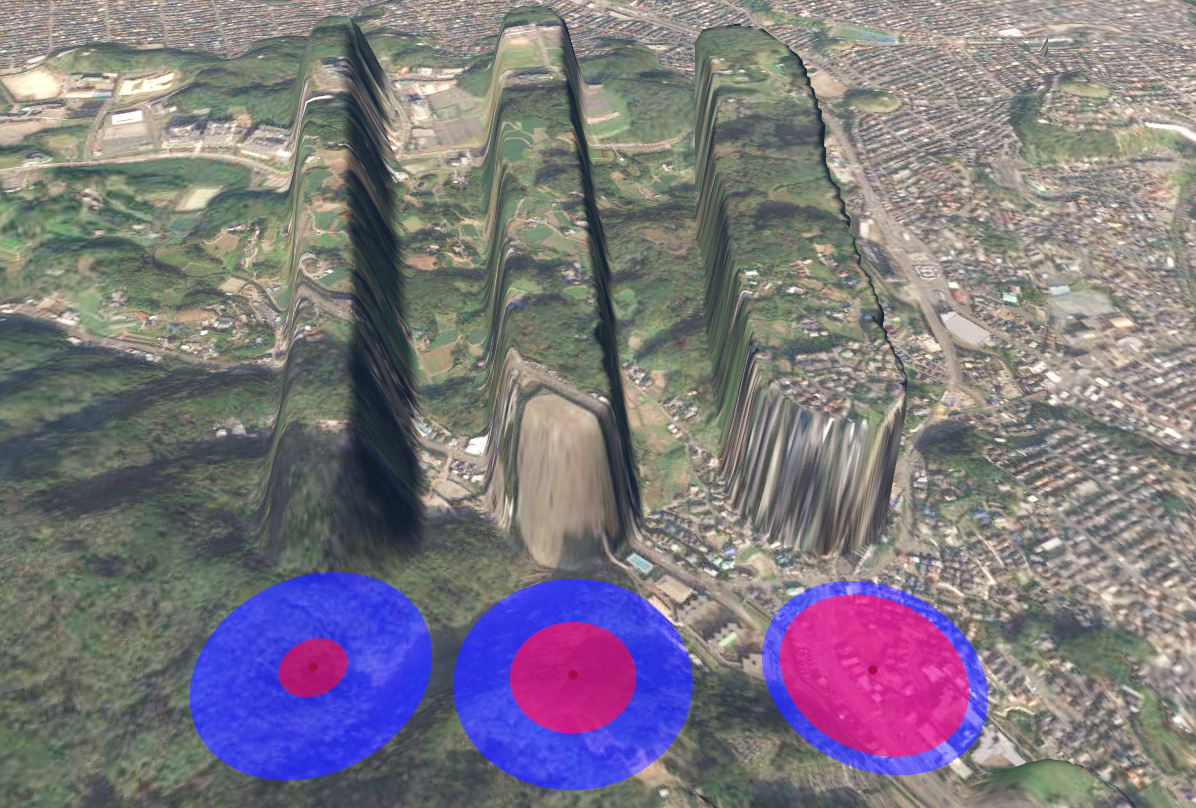
\includegraphics[height=4cm        ,width=5cm]{figures/flatten2.jpg}
\caption{三种不同的笔刷内直径编辑的效果}
\end{figure}
为保证编辑操作的合理性,笔刷可设置的编辑高度区间在[-1000,1000]之间,笔刷最大直径为6千米左右,最高可在分层四叉树的第10层进行编辑。
\section{基于选区的地形高程编辑}
由于地形高程数据精度有限且存在误差,可能会在地表局部产生凹凸不平、尖刺和坑洞的现象。对于机场、城市等有近地漫游需求且需要地面平整来摆放模型的应用场景来说,需要提供一种编辑工具可以快速对地面进行平整。考虑到操作效率和简便程度,对地形块进行选区操作比笔刷涂抹更好。此外,还可以通过框选对地形进行腐蚀操作,腐蚀是模拟物理世界中水土流失的规律的技术,经过多次迭代后产生的效果可以很大的提升地型真实感。由于腐蚀操作需要进行数十次到数百次的迭代,因此在GPU端的实现更适应实时编辑的要求。地形平滑等功能需要对地形数据进行卷积滤波,也需要多次迭代以达到较好的效果。为了架构的清晰,地形平滑采用了和腐蚀一样的工作管线。\par
选区操作的实现特点是将地形高程数据采样为一张纹理图,在GPU中进行处理。这种方式打破了着色器只能更新当前所处理顶点的数据、无法访问同一网格中其他顶点的数据的限制,使腐蚀、平滑等需要获取某点邻域中的地形数据的算法得以实现。在得到补丁数据后,将补丁数据作为纹理传入GPU,由于地形高程数据的分辨率是2的幂,补丁数据的传输对图形硬件较为友好。经过片元着色器的运算后,将补丁数据渲染在一个UV值在$[0,1]$间的简单四边形面片上。将OpenGL视口的宽高设置为补丁数据的宽高,以使输入输出图片分辨率相等。用一个附加纹理的帧缓存作为接收结果数据的对象,在多次迭代中使用两个纹理交替做为输入和输出。\par
选区范围由鼠标在地形上点选拖拽生成,起点为鼠标按下左键开始拖拽的点,终点为拖拽结束松开鼠标的点。以分层四叉树最精细层级对地形块进行选择,与选区有交集的所有地形块都会被选中,一个地形块或者完全被选中,或者完全不被选中。为显示用户选择的选区范围,在鼠标拖拽时要实时绘制当前所选择到的选区边界。鼠标拖拽时鼠标当前所在经纬度被实时更新,选区边界以选区左下角和右上角的经纬度确定。由于经纬度向地形块索引的转换是向下取整的,地形块坐标系统的$x$和$y$值分别向右向上递增,原点在地图的左下角,因此对于地形块内的所有点,根据其经纬度计算索引,该索引转换为经纬度所在的点在该地形块的左下角,左下角的经纬度得以确认。对选区右上角的地形块索引的$x$、$y$值加1进行矫正,即索引为$(x,y,level)$的地形块的右上角即为索引为$(x+1,y+1,level)$的地形块的左下角。然后根据地形块索引和地形块所在层级每个块的经纬度尺寸,获取地形块左下角的数据,分别绘制选区的四条边。由于四叉树分裂算法的性质,多数时间视野中的地形块数量较少,但出于图形硬件的限制和对操作效率的考虑,还是对地形选区可框选的块数和选区所在层数进行了限制。\par
高程数据可以以高度图的形式表示,地形平滑可以看作对高度图进行平滑滤波,使高度图变得模糊,并消除图中的噪点。反映在地形上则减少了地形上某点与其邻域的高程差,消除了与邻域高程差过大的点。平滑滤波通常取相邻像素点的值,按固定权重进行平均,随着邻域的扩大,平滑效果会得到增强,但也存在边际递减效应。考虑到进行图片采样的时间消耗,系统中取目标像素八邻域内的像素,简单进行平均,可以取得较好的效果。由于只对高程数据进行改变,地表纹理数据中因高程起伏产生的阴影无法消除,视觉效果上依然存在不平整的感觉。但考虑到此功能的应用场景多为城市、机场跑道等建筑区域,且主要目的是为了更好的摆放模型、去除高程数据中的噪点,上述的缺陷是可以接受的。


\section{结果分析}
本系统中的用户界面由Qt框架支持,高程编辑器界面设计如图4.4所示,使用时通过最上面的功能按钮切换当前使用的功能,并通过滑动条对当前功能提供的可调参数进行调整。通过点击下方的按钮可以进行操作撤销和重做,编辑结束后可以对编辑工程进行保存,也可以将编辑结果导出至数据库。图4.5展示了ViWo系统中旧地形编辑器的编辑界面。旧地形编辑器需要在进入编辑状态时固定编辑层级和编辑范围,本编辑器可以在浏览和编辑状态间无缝切换,可以更方便的从不同视角、不同层级进行编辑。
\begin{figure}[htbp]
    \centering
    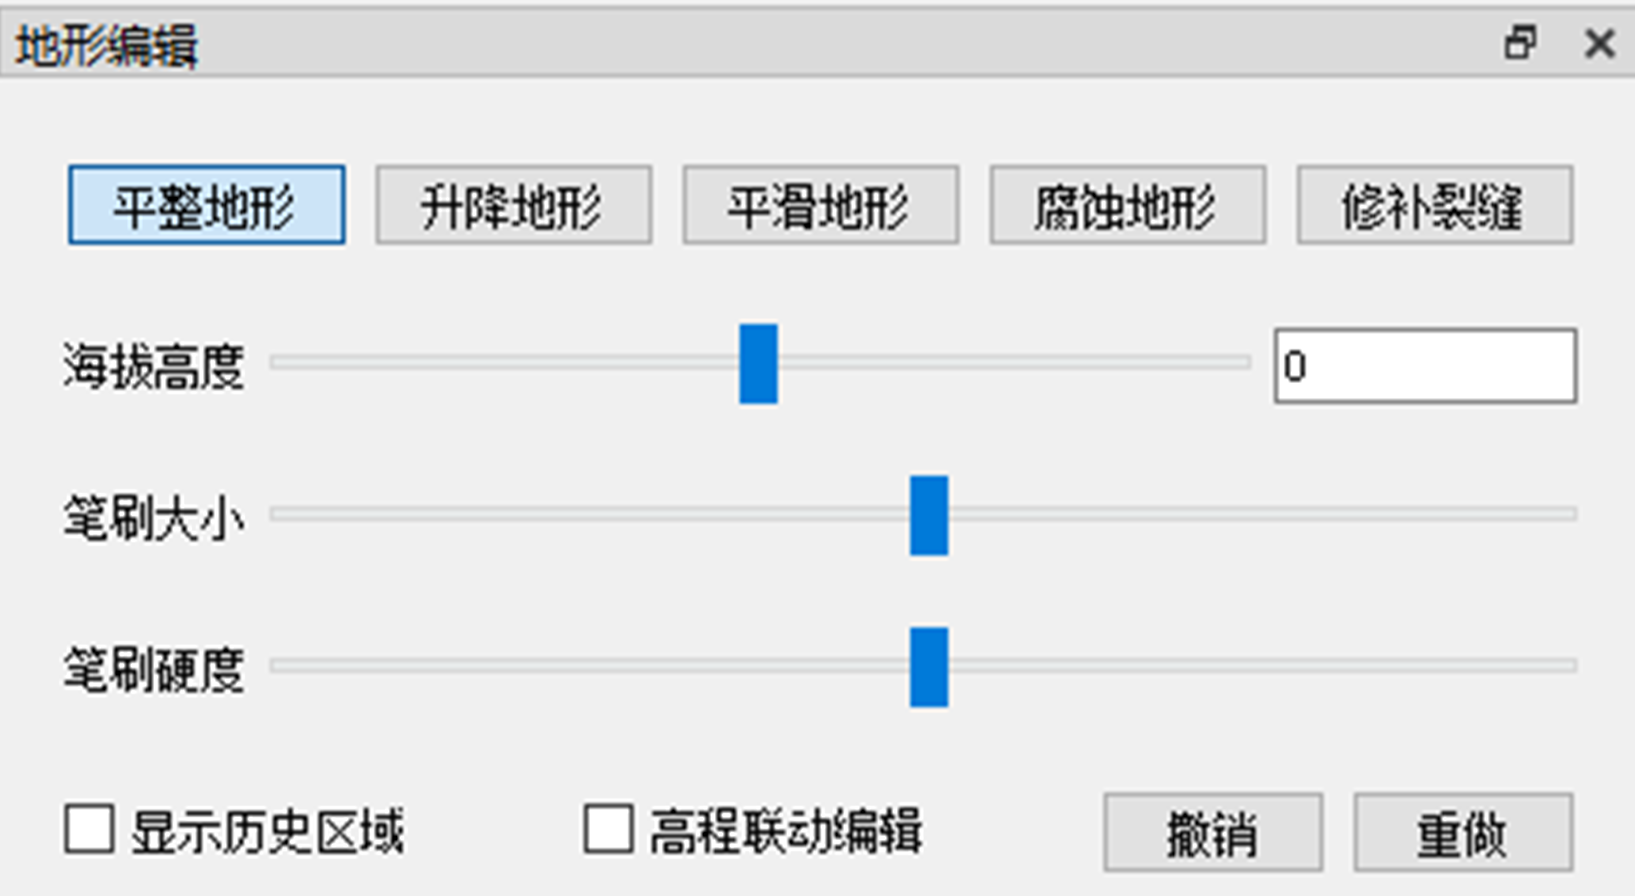
\includegraphics[height=4.9cm,width=8.6cm]{figures/demInterface.png}
  \caption{高程编辑器界面}
  \end{figure}
  
  \begin{figure}[h]
\centering
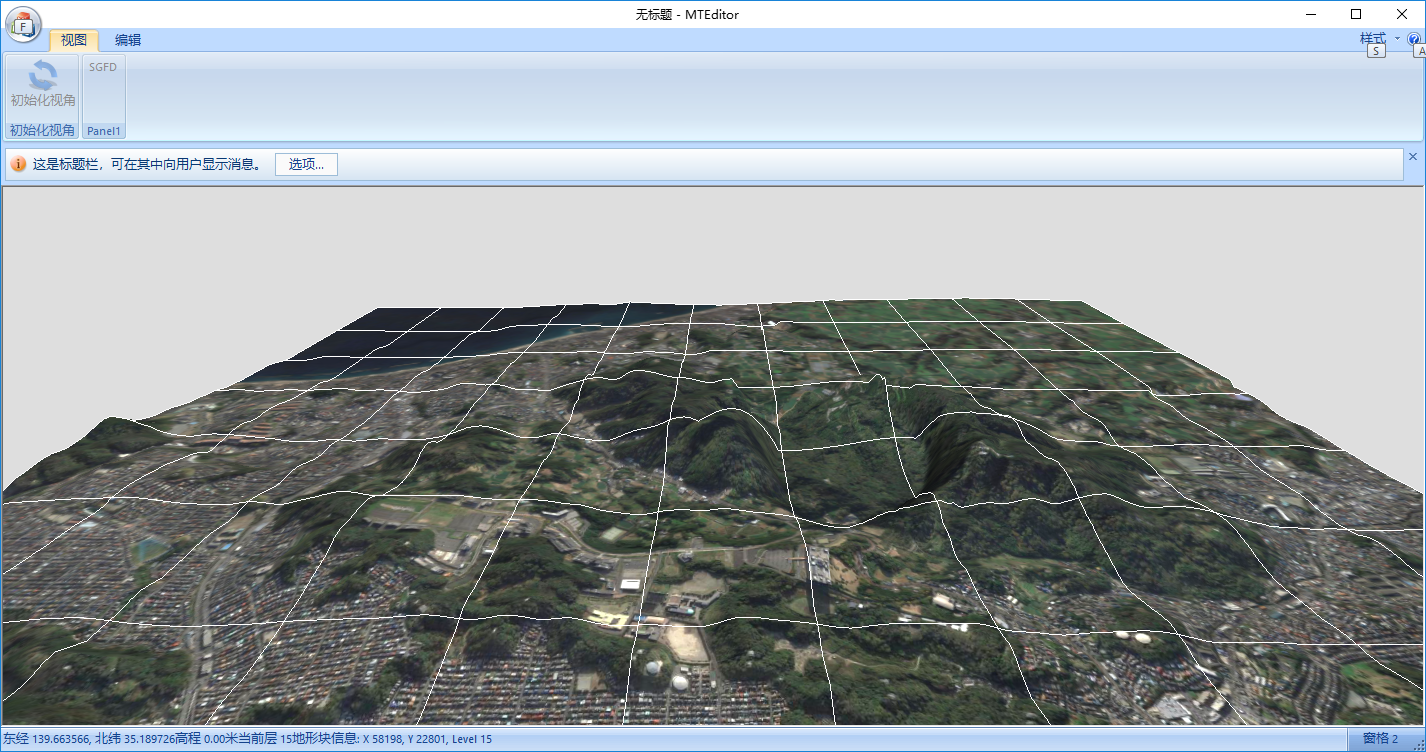
\includegraphics[height=4.2cm        ,width=7.2cm]{figures/old.png}
\caption{ViWo系统中旧编辑器编辑状态效果}
\end{figure}
图4.6展示了本编辑器中以选区方式进行地形平滑操作的过程,平滑前选区包含了三条笔刷绘制出的山脉,平滑后选区边界的高程得到了良好的保持,且与选区区域内部过渡自然。旧地形编辑器中不具备地形选区的概念,当进行地形腐蚀操作时,直接对编辑范围内的地形进行操作,因此交互上可能会产生更大的延迟。par

\begin{figure}[htbp]
\centering
\subcaptionbox{}{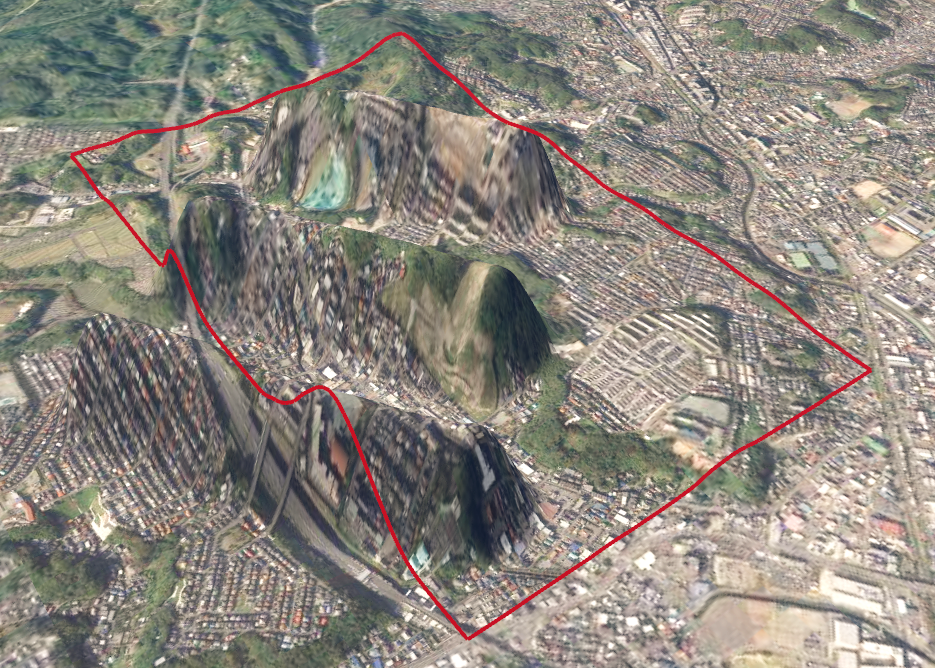
\includegraphics[height=3.5cm        ,width=6.8cm]{figures/areaSmooth-.PNG}}
\subcaptionbox{}{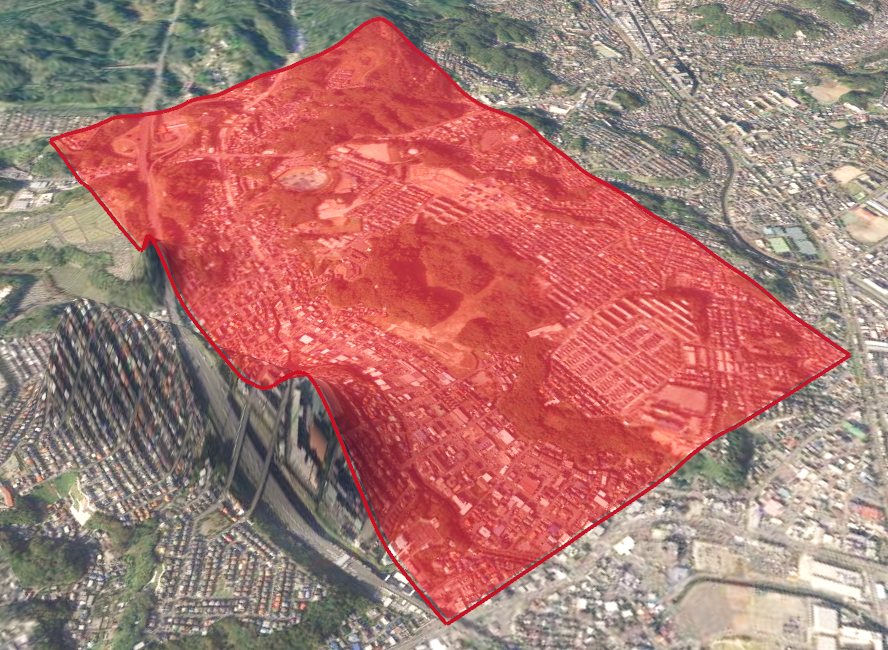
\includegraphics[height=3.5cm        ,width=6.8cm]{figures/areaSmooth-2.PNG}}\\
%\subcaptionbox{}{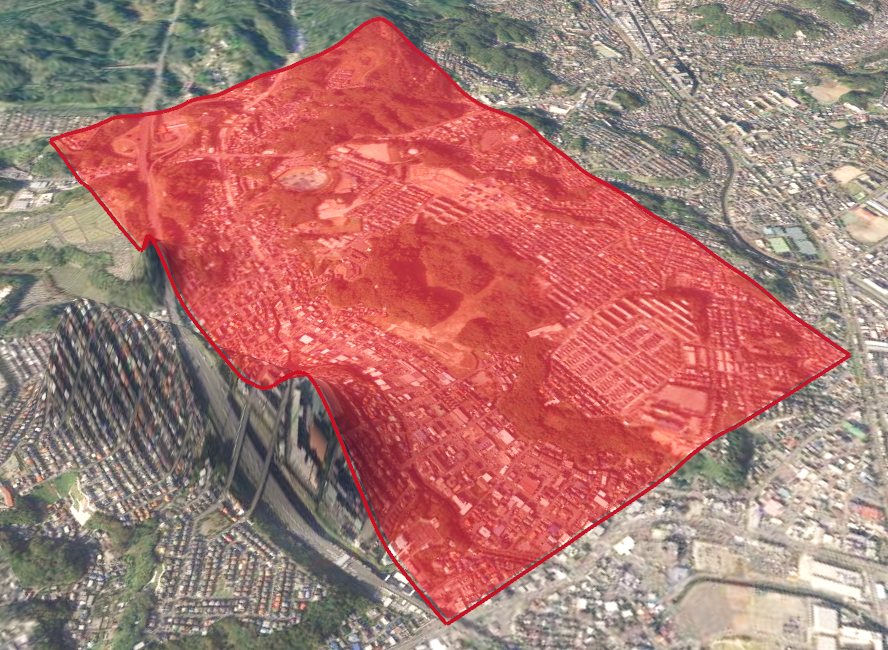
\includegraphics[height=4.5cm        %,width=7.2cm]{figures/areaSmooth-2.PNG}}

\caption{在两种不同视角下对地形平滑结果的观察:(a).平滑前(b).平滑后}
\end{figure}

北京国遥新天地公司研发的EV-Globe6.0系统\supercite{ev-globe}是目前较为活跃的基于分层四叉树提供地形编辑功能的地形系统。图4.7对比了EV-Globe6.0与本编辑器实现的高程画刷编辑、平整编辑效果。本编辑器的画刷绘制了画刷中心点,对用户的提示效果更明确。EV-Globe6.0中的画刷贴合在地形表面,对画刷覆盖下的地形可以观察的更清楚。地形升降的效果上,两个系统基本相同。在地形平整功能上,EV-Globe6.0采用了矢量线编辑,编辑出的梯田地形边缘清晰锐利,锯齿很少。本编辑器对平整边缘进行了平滑,平整区域和未平整区域的过渡更加自然。使用本编辑器进行完整地形编辑的效果详见附录。\par

\begin{figure}[h]
\centering
\subcaptionbox{}{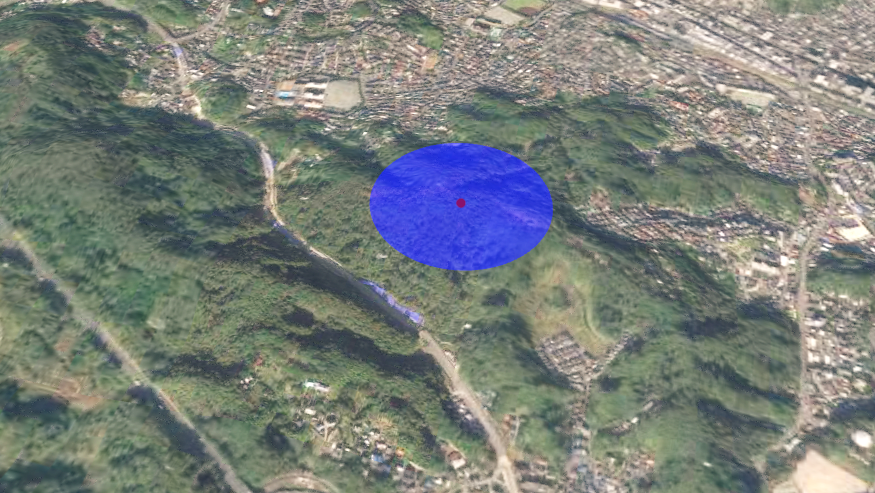
\includegraphics[height=2.8cm        ,width=4.6cm]{figures/heightBefore.png}}
\subcaptionbox{}{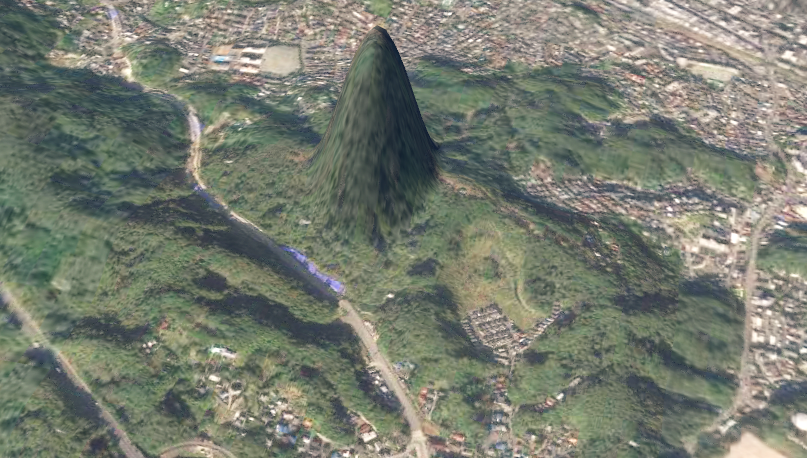
\includegraphics[height=2.8cm        ,width=4.6cm]{figures/heightAfter.png}}\\
\subcaptionbox{}{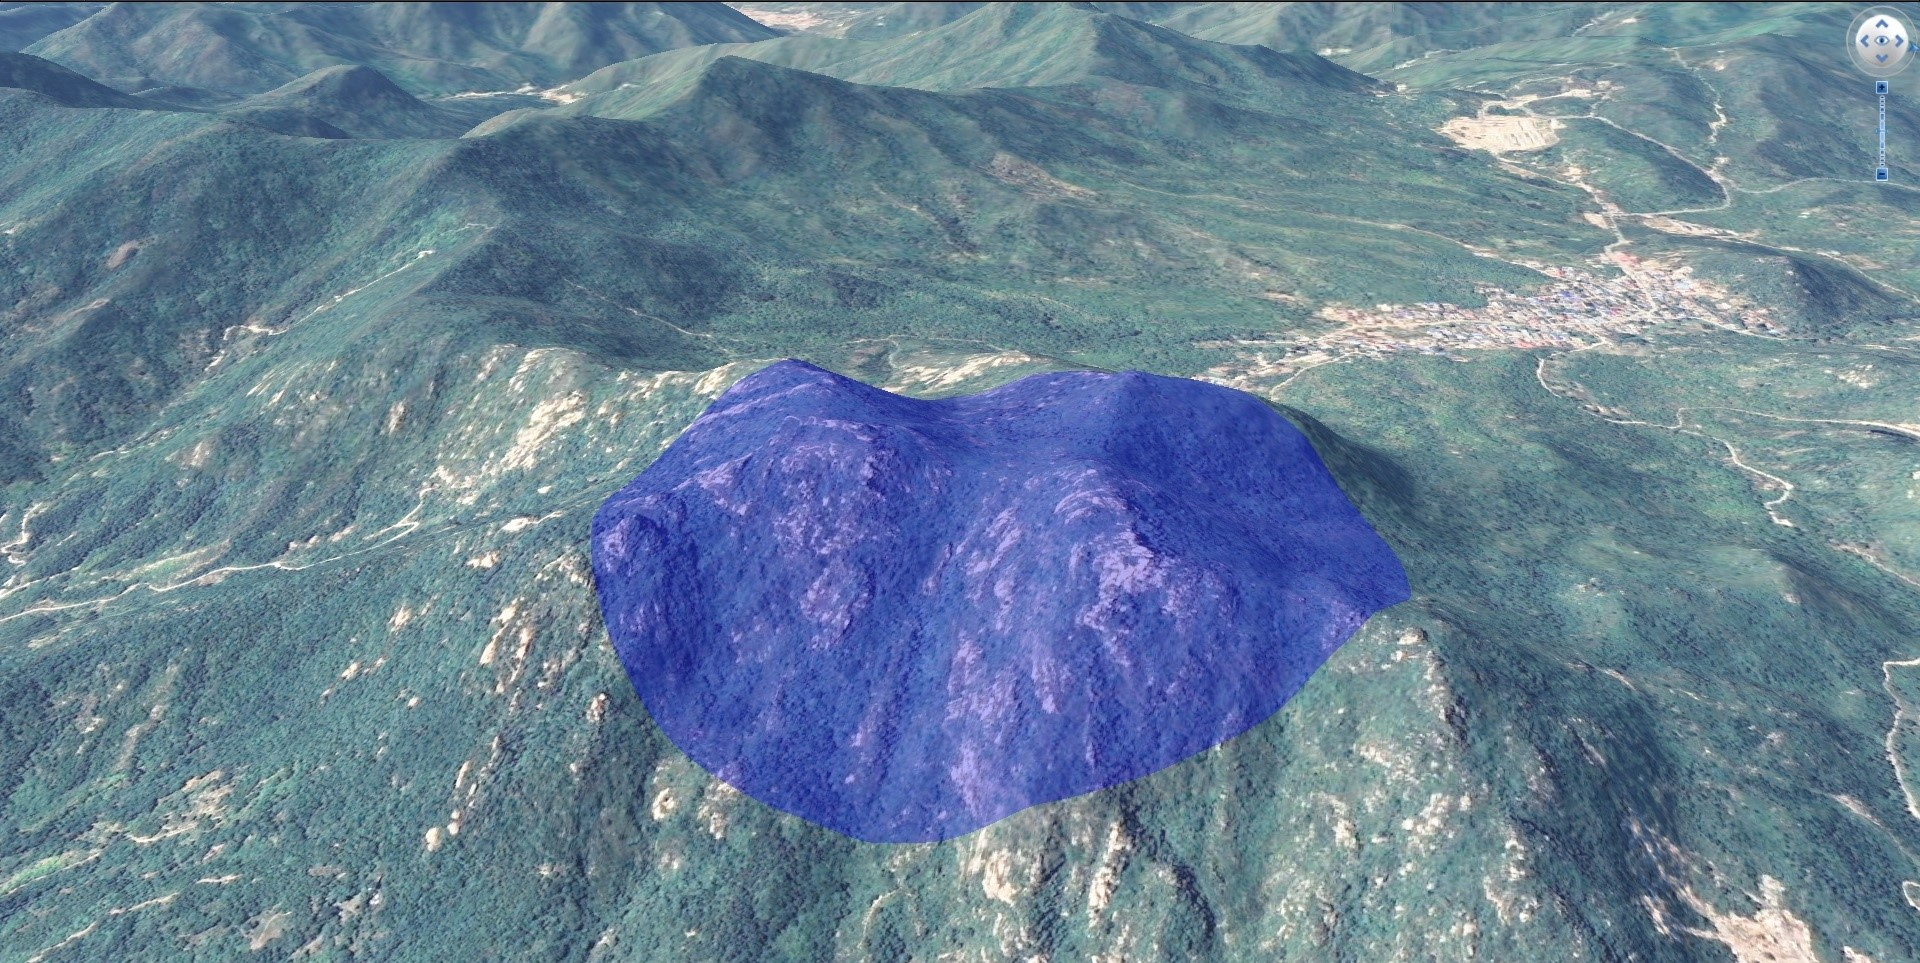
\includegraphics[height=2.8cm        ,width=4.6cm]{figures/demBefore.jpg}}
\subcaptionbox{}{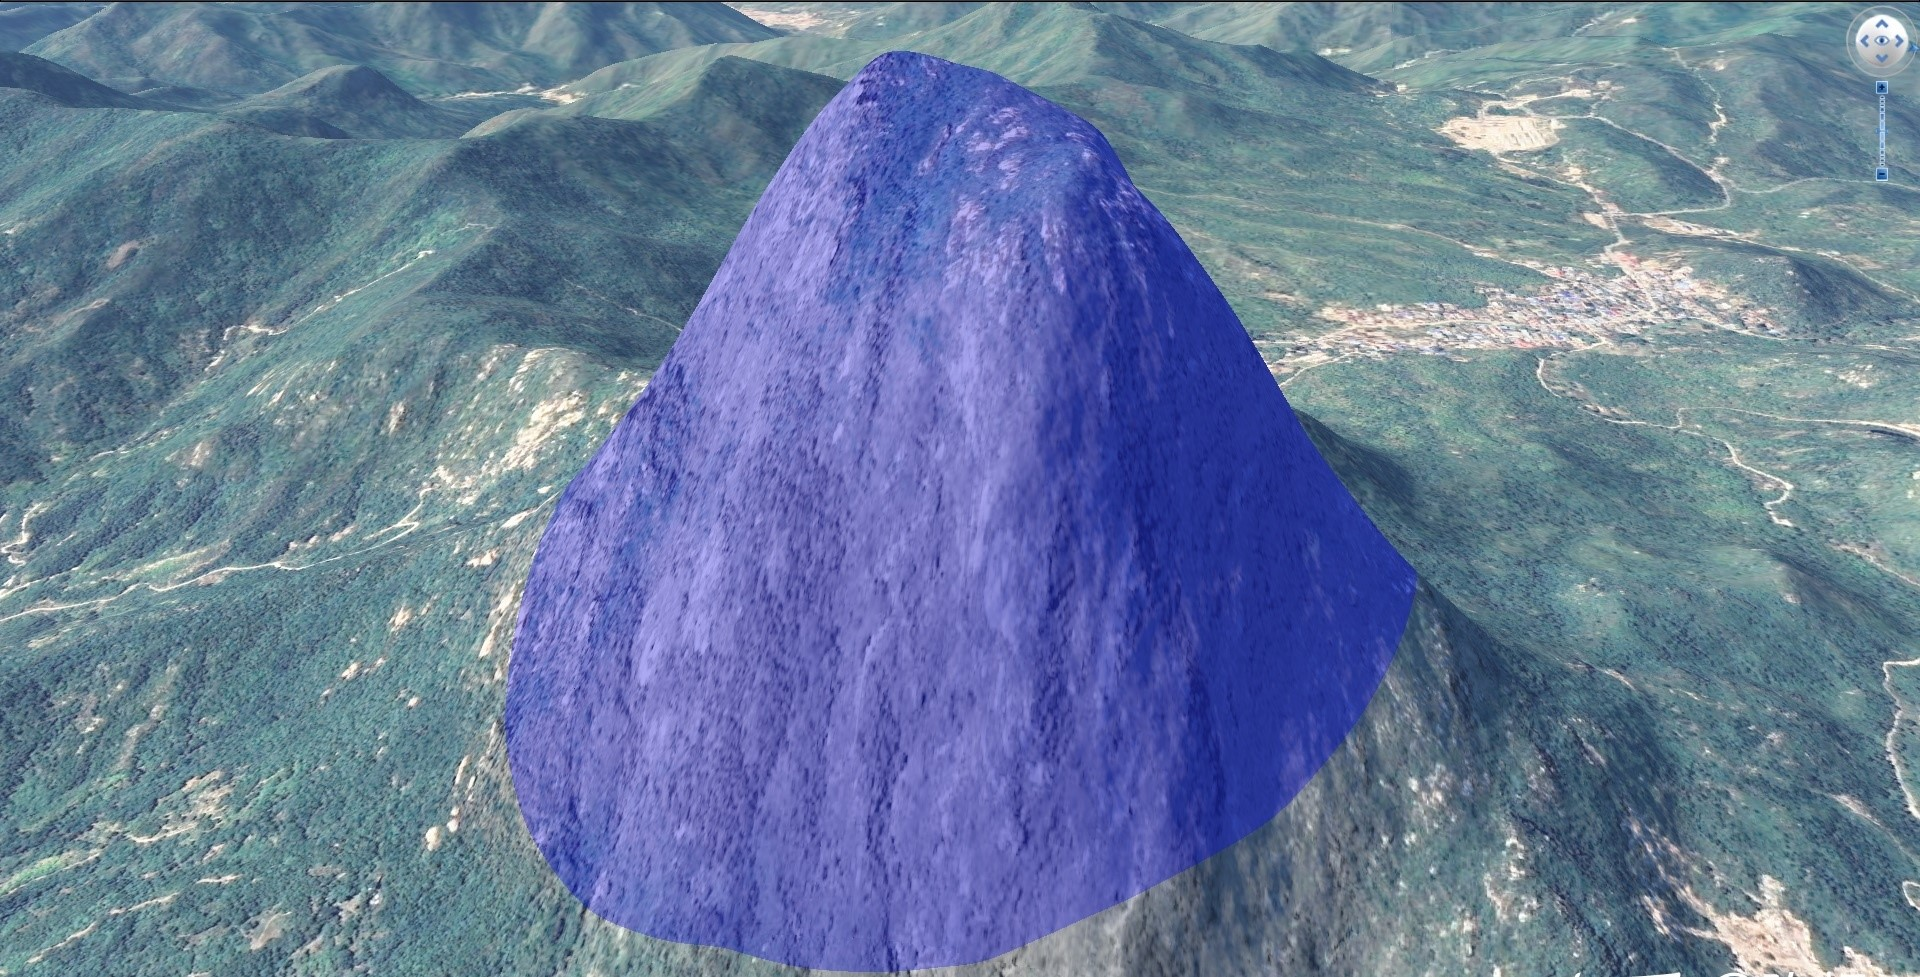
\includegraphics[height=2.8cm        ,width=4.6cm]{figures/demAfter.jpg}}\\
\subcaptionbox{}{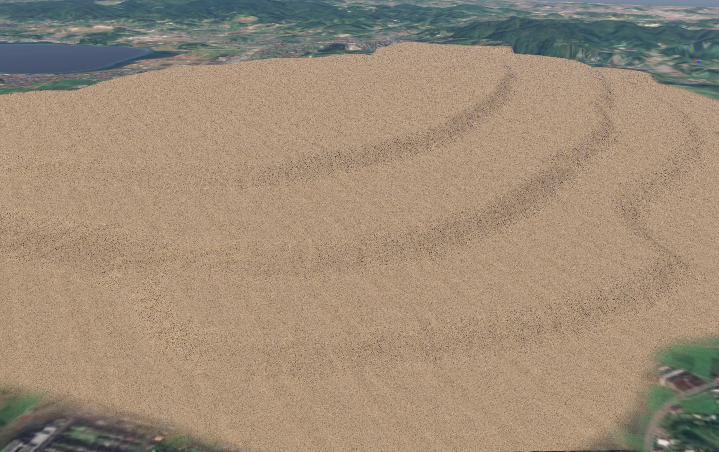
\includegraphics[height=2.8cm        ,width=4.6cm]{figures/mytitian2.PNG}}
\subcaptionbox{}{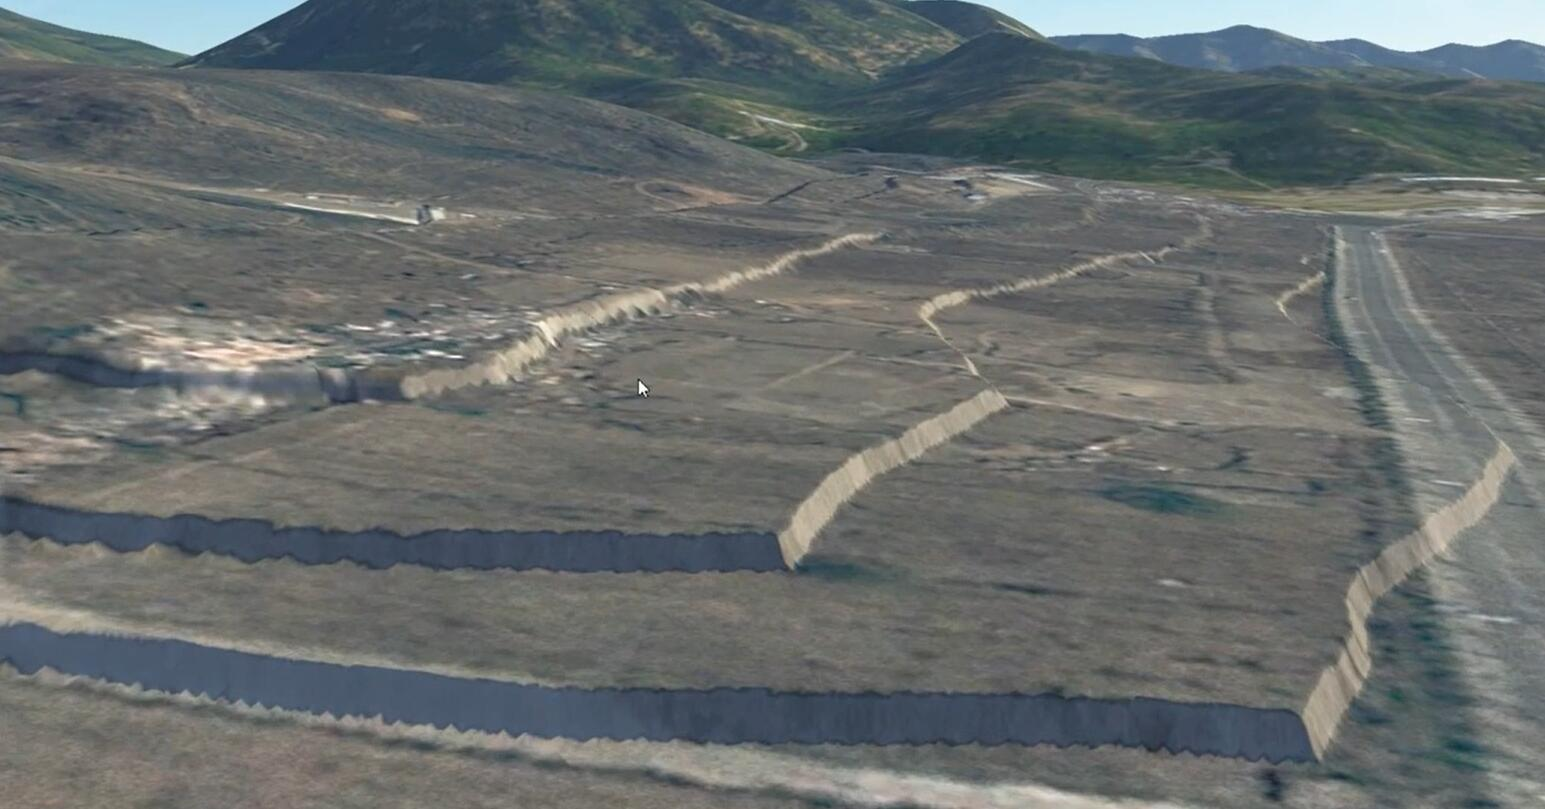
\includegraphics[height=2.8cm        ,width=4.6cm]{figures/titianEv.jpg}}

\caption{EV-Globe6.0与本编辑器效果对比\supercite{ev-globe}:(a).ViWo高程编辑前(b).ViWo高程编辑后(a).EV-Globe6.0高程编辑前(b).EV-Globe6.0高程编辑后(c).ViWo平整编辑后(d).EV-Globe6.0平整编辑后}
\end{figure}
\section{本章小结}
本章介绍了编辑器中实现地形高程编辑的方法,包括使用笔刷和选区两种工具对地形进行平整、平滑等操作的算法。其中详细阐述了笔刷和选区编辑范围的确定,编辑结果的计算方法,并给出了实验结果。\par

% vim:ts=4:sw=4
